\documentclass[a4paper,oneside]{memoir}
\usepackage{standalone}
\usepackage[utf8]{inputenc}
\usepackage[british]{babel}
\usepackage{csquotes}
\usepackage[T1]{fontenc}
\usepackage{charter}
\usepackage[bitstream-charter]{mathdesign}
\usepackage[final,babel]{microtype}
\usepackage{siunitx}
\usepackage{amsmath}
\usepackage{bm}
\usepackage{mathtools}
\usepackage{subcaption}
\usepackage{booktabs}
\usepackage{xcolor}
\PassOptionsToPackage{final}{graphicx}
\usepackage{tikz}
\usepackage{blindtext}
\usepackage{natbib}
\usepackage[colorlinks,linkcolor=blue,citecolor=blue,urlcolor=blue]{hyperref}
\usepackage{doi}
\usepackage{bookmark}
\usepackage{pifont}
\usepackage{makecell}

\sisetup{round-mode=off,round-precision=3}

\usetikzlibrary{plotmarks}
\usetikzlibrary{patterns}

% https://tex.stackexchange.com/q/139401/23339
\graphicspath{{src/thesis/}{build/}}

% https://tex.stackexchange.com/a/79060/23339
\makeatletter
\def\input@path{{src/thesis/}{build/thesis/}{build/}}
\makeatother

% http://tex.stackexchange.com/q/135352/23339
\makeatletter
\def\hrulefill{\leavevmode\leaders \hrule height \rulethickness \hfill\kern\z@}
\makeatletter

% https://tex.stackexchange.com/q/156048/23339
% https://tex.stackexchange.com/q/207905/23339
\newcommand{\inputval}[1]{\protect\input{#1}\ignorespaces}

\newcommand{\TODO}[1]{\textcolor{purple}{TODO: \emph{#1}}}
\newcommand{\vect}{\mathbf}
\newcommand{\uf}{\vect{u}_f}
\newcommand{\Opp}{\mathrm{Opp}}
\newcommand{\Sf}{\vect{S}_f}
\newcommand{\Mag}[1]{\lvert #1 \rvert}
\newcommand{\magSf}{\Mag{\Sf}}
\newcommand{\vol}{\mathcal{V}}


\setlrmarginsandblock{\spinemargin}{1in}{*}
\setmarginnotes{0in}{0in}{0in}
\checkandfixthelayout

\renewcommand{\cellalign}{tl}

\title{Numerical representation of mountains in atmospheric models}
\author{James Shaw}
\date{\TODO{date}}

\makeatletter
\AtBeginDocument{
  \hypersetup{
    pdftitle = {\@title},
    pdfauthor = {\@author}
  }
}
\makeatother

\OnehalfSpacing
\makechapterstyle{mysouthall}{%
% https://tex.stackexchange.com/a/309189/23339
\newlength{\aftertocskip}
\setlength{\aftertocskip}{2.7\baselineskip}% Space after ToC title
\renewcommand*{\aftertoctitle}{%
\par\vspace{\baselineskip}%
\hrulefill \par\nobreak\noindent \vskip\aftertocskip}
\setlength{\afterchapskip}{5\baselineskip}
\setlength{\beforechapskip}{36pt}
\setlength{\midchapskip}{\textwidth}
\addtolength{\midchapskip}{-\beforechapskip}
\renewcommand*{\chapterheadstart}{\vspace*{2\baselineskip}}
\renewcommand*{\chaptitlefont}{\huge\rmfamily\raggedright}
\renewcommand*{\chapnumfont}{\chaptitlefont}
\renewcommand*{\printchaptername}{}
\renewcommand*{\chapternamenum}{}
\renewcommand*{\afterchapternum}{}
\renewcommand*{\printchapternum}{%
\begin{minipage}[t]{\beforechapskip}
{\vspace{0pt}\chapnumfont%%%\figureversion{lining}
\thechapter}
\end{minipage}}
\renewcommand*{\printchaptertitle}[1]{%
\hfill\begin{minipage}[t]{\midchapskip}
{\vspace{0pt}\chaptitlefont ##1\par}\end{minipage}}
\renewcommand*{\afterchaptertitle}{%
\par\vspace{\baselineskip}%
\hrulefill \par\nobreak\noindent \vskip\afterchapskip}}
\chapterstyle{mysouthall}

\captionnamefont{\small}
\captiontitlefont{\small}

\begin{document}
\begin{titlingpage}
\makeatletter
\begin{center}
\textsc{\Large University of Reading} \\[12pt]
{\Large Department of Meteorology} \\[16pt]
\includegraphics{img/uor-logo} \\[48pt]

\rule{\textwidth}{.4pt} \\[12pt]
{ \huge \bfseries \@title \\[16pt] } \rule{\textwidth}{.4pt} \\[54pt]
{\LARGE \@author}
\vfill
{\Large \@date}
\end{center}
\makeatother
\end{titlingpage}


\frontmatter
\thispagestyle{plain}
\null\vfil
\begin{abstract}
\blindtext
\end{abstract}
\vfil

\cleardoublepage
{\hypersetup{linkcolor=black}\tableofcontents*}

\mainmatter
\chapter{Introduction}
\chapter{Existing methodologies}
\chapter{Numerically stable transport over steep slopes}
\label{ch:cubicFit}

\begin{highlights}
{\Large Highlights}
\begin{itemize}
	\item The new cubicFit transport scheme is second-order convergent regardless of mesh distortions or the choice of velocity field
	\item Sub-grid reconstructions are mostly precomputed depending on the mesh geometry alone
	\item Misalignment of the velocity field with mesh layers is the primary source of numerical error, not simply mesh distortions
\end{itemize}
\end{highlights}

\TODO{
Motivation
\begin{itemize}
	\item Conservation of tracer, therefore Eulerian
	\item Numerically stable and accurate on arbitrary meshes (because no consensus on "best" mesh: hex or cubed-sphere? TF or cut cells?)
	\item Avoid all splitting errors (because they get worse with steeper slopes represented by TF meshes)
	\item Method-of-lines approach permits low computational cost
\end{itemize}
}

\section{Transport schemes for arbitrary meshes}
\label{sec:cubicFit:transport}

The transport of a tracer density $\phi$ in a prescribed, non-divergent velocity field $\vect{u}$ is given by the flux-form equation \citep{nair-lauritzen2010}
\begin{align}		
	\frac{\partial \phi}{\partial t} + \nabla \cdot \left( \vect{u} \phi \right) = 0 \text{ .} \label{eqn:advection}		
\end{align}
The time derivative is discretised using an explicit, two-stage, second-order Heun scheme,
\begin{subequations}
\begin{align}
	\phi^\star &= \phi^{(n)} + \Delta t \: g(\phi^{(n)}) \\
	\phi^{(n+1)} &= \phi^{(n)} + \frac{\Delta t}{2} \left[ g(\phi^{(n)}) + g(\phi^{\star}) \right]
\end{align} \label{eqn:heun}%
\end{subequations}
\unskip where \(g(\phi^{(n)}) = - \nabla \cdot (\vect{u} \phi^{(n)})\) at time level \(n\).
This two-stage second-order time-stepping scheme is similar to the three-stage second-order time-stepping scheme used later in a model of the fully compressible Euler equations (section~\ref{sec:slanted:exnerFoamH}), which needs an additional time-stage to converge upon the semi-implicit solution.
The two-stage second-order time-stepping scheme is used for both the cubicFit scheme and the multidimensional linear upwind scheme.
Although the Heun scheme is unstable for a linear oscillator \citep{durran2013} and for solving the transport equation using centred, linear differencing, it is stable when it is used for transport schemes with sufficient upwinding \citep[p. 149]{hundsdorfer-verwer2013}.

Using the finite volume method, the velocity field is prescribed at face centroids and the dependent variable is stored at cell centroids.  The divergence term in equation~\eqref{eqn:advection} is discretised using Gauss's theorem,
\begin{align}
	\nabla \cdot \left( \vect{u} \phi \right) \approx \frac{1}{\vol_c} \sum_{f \in\:c} \vect{u}_f \cdot \Sf \phi_F \label{eqn:gauss-div}
\end{align}
where subscript $f$ denotes a value stored at a face and subscript $F$ denotes a value approximated at a face from surrounding values.  $\vol_c$ is the cell volume, $\vect{u}_f$ is a velocity vector prescribed at a face, $\Sf$ is the surface area vector with a direction outward normal to the face and a magnitude equal to the face area, $\phi_F$ is an approximation of the dependent variable at the face, and $\sum_{f \in\:c}$ denotes a summation over all faces $f$ bordering cell $c$.

This discretisation is applicable to arbitrary meshes.  A necessary condition for stability is given by the multidimensional Courant number \citep{weller-shahrokhi2014},
\begin{align}
	\mathrm{Co}_c = \frac{\Delta t}{2 \mathcal{V}_c} \sum_{f \in\: c} \Mag{\vect{u} \cdot \Sf} \label{eqn:co}
\end{align}
such that, for all cells $c$ in the domain, $\mathrm{Co}_c$ is less than or equal to some constant that depends upon the spatial and temporal discretisation.  Hence, stability is constrained by the maximum Courant number of any cell in the domain.

The accurate approximation of the dependent variable at the face, $\phi_F$, is key to the overall accuracy of the transport scheme. The cubicFit scheme and the multidimensional linear upwind scheme differ in their approximations, and these approximation methods are described next.


\section{High-order finite volume formulation}
\label{sec:highOrderFit:scheme}

Integrating the flux-form transport equation \eqref{eqn:advection} over a volume $\vol$ and using Gauss's divergence theorem,
\begin{align}
	\int_\vol \frac{\partial \phi}{\partial t} d\vol = - \int_{\partial \vol} \phi \vect{u} \cdot \unitn dA \label{eqn:highOrder:integrated-advection}
\end{align}
where $\unitn$ is the outward unit normal vector.
Using the method of lines, the time derivative is discretised using the classical fourth-order Runge–Kutta time-stepping scheme \citep[p. 53]{durran2013}, and the spatial discretisation is described next.
For a polygonal cell with faces $f$ equation~\eqref{eqn:highOrder:integrated-advection} becomes
\begin{align}
	\int_\vol \frac{\partial \phi}{\partial t} d\vol = - \sum_f \int_{\area_f} \phi \vect{u} \cdot \unitn d\area_f \label{eqn:highOrder:advection}
\end{align}
where $\area_f$ is the area of face $f$.
If $\phi$ is a sufficiently smooth field then it can be approximated to $P$-order accuracy by replacing $\phi$ with a polynomial interpolant $\psi$,
\begin{align}
	\psi = \sum_{\Mag{\vect{p}} \leq P} a_{\vect{p}} \left(\vect{x} - \vect{x}_0 \right)^\vect{p} \label{eqn:highOrder:interpolant}
\end{align}
where $a_\vect{p}$ are unknown polynomial coefficients, $\vect{x}_0$ is a fixed position, and $P$ is the total polynomial order.
Note that we use the multi-index notation such that $\Mag{\vect{p}} = p_1 + \ldots + p_n$ and
\begin{align}
	a_{\vect{p}} \left( \vect{x} - \vect{x}_0 \right)^\vect{p} = a_\vect{p} \prod_{d=1}^D \left( x_d - x_{0_d} \right)^{p_d} \text{ .}
\end{align}
where $D$ is the number of physical dimensions.
As an example, the exponents $\vect{p}$ in two dimensions $(x, y)$ with $\Mag{\vect{p}} \leq 1$ are $(0, 0)$, $(1, 0)$ and $(0, 1)$, hence the two-dimensional polynomial interpolant for a total polynomial order $P = 1$ is
\begin{align}
	\psi = a_{0,0} + a_{1,0} \left( x - x_0 \right) + a_{0,1} \left( y - y_0 \right) \text{ .}
\end{align}
Replacing $\phi$ in \eqref{eqn:highOrder:advection} with $\psi$ in \eqref{eqn:highOrder:interpolant} we obtain an expression for the face flux,
\begin{align}
	\int_\area \phi \vect{u} \cdot \unitn d\area = \uf \cdot \unitn \sum_{\Mag{\vect{p}} \leq P} a_{\vect{p}} \moment_\area^\vect{p} \label{eqn:highOrder:face-flux}
\end{align}
where $\moment_\area^\vect{p} = \int_\area \left( \vect{x} - \vect{x}_0 \right)^\vect{p} d \area$ is the $\vect{p}$-th moment of area $\area$.
\TODO{here we're assuming that $\vect{u}$ is smoother than $\phi$, see \citet{methven-hoskins1999} for a justification?}
Therefore, the face flux can be calculated by finding the the polynomial coefficients $a_\vect{p}$.

Following the same approach as the cubicFit transport scheme, taking a total polynomial order $P = 3$ gives 9 polynomial terms with polynomial coefficients calculated using the same upwind-biased stencil.
For every cell in the stencil we require that the average of the polynomial integrated over a cell volume equals the cell average value,
\begin{align}
	\volave{\psi} = \volave{\phi} \label{eqn:highOrder:equal-volumes}
%
\intertext{where the average over volume $\vol$ is}
%
	\volave{\psi} = \frac{1}{\vol} \int_\vol \psi d\vol \text{ .} \label{eqn:highOrder:volume-average}
\end{align}
Using equations~\eqref{eqn:highOrder:interpolant} and \eqref{eqn:highOrder:volume-average} we can rewrite equation~\eqref{eqn:highOrder:equal-volumes} as
\begin{align}
	\frac{1}{\moment_\vol^\vect{0}} \sum_{\Mag{\vect{p}} \leq P} a_\vect{p} \moment_\vol^\vect{p} = \volave{\phi}
\end{align}
where $\moment_\vol^\vect{p} = \int_\vol \left( \vect{x} - \vect{x}_0 \right)^\vect{p} d\vol$ is the $\vect{p}$-th moment of volume $\vol$, and the zeroth moment $\moment_\vol^\vect{0}$ is the volume.
For $m$ polynomial terms and a stencil with $n$ cells, we calculate a face flux by choosing $\vect{x}_0$ to be the position of the face centre, then we write the linear system
\begin{align}
	\begin{bmatrix}
		\moment_{\vol_1}^{\vect{p}_1}/\moment_{\vol_1}^\vect{0} & \cdots & \moment_{\vol_1}^{\vect{p}_m}/\moment_{\vol_1}^\vect{0} \\
		\vdots & & \vdots \\
		\moment_{\vol_n}^{\vect{p}_1}/\moment_{\vol_n}^\vect{0} & \cdots & \moment_{\vol_n}^{\vect{p}_m}/\moment_{\vol_n}^\vect{0}
	\end{bmatrix}
	\begin{bmatrix}
		a_{\vect{p}_1} \\
		\vdots \\
		a_{\vect{p}_m}
	\end{bmatrix}
	=
	\begin{bmatrix}
		\langle \phi \rangle_{\vol_1} \\
		\vdots \\
		\langle \phi \rangle_{\vol_n}
	\end{bmatrix} \label{eqn:highOrder:moment-matrix}
\end{align}
which can be written as
\begin{align}
	\vect{B} \vect{a} = \bm{\phi} \text{ .}
\end{align}
where $\vect{B}$ is the stencil matrix, which is constructed using only the mesh geometry.
The highOrderFit scheme generates stencils using the same procedure as the cubicFit scheme.
Assuming a stencil comprises at least as many cells as there are polynomial coefficients then $n \geq m$ and the matrix equation can be solved using a least-squares approach to find the unknown coefficients $\vect{a}$.

To obtain a stable transport scheme, we follow the approach of the cubicFit scheme by introducing multipliers $\vect{m}$ to obtain
\begin{align}
	\vect{\tilde{B}} \vect{a} = \vect{m} \cdot \bm{\phi}
\end{align}
where $\vect{\tilde{B}} = \vect{M} \vect{B}$ and $\vect{M} = \mathrm{diag}(\vect{m})$.
The upwind cell and downwind cell have multipliers $m_u = 2^{10}$ and $m_d = 2^{10}$ respectively, and all peripheral points have multipliers $m_p = 1$.

The calculation of high-order cell volume moments and surface moments are required by equations~\eqref{eqn:highOrder:moment-matrix} and~\eqref{eqn:highOrder:face-flux} respectively.  These volume and surface moments can be calculated exactly using the method of \citet{tuzikov2003}.
We follow their method but, in order to avoid any degenerate triangles, we introduce a centre point shared by all triangles instead of triangulating polygons with only existing vertices.

While the highOrderFit transport scheme uses a total polynomial order $P = 3$ for stencils in the domain interior, a total polynomial order $P = 1$ is used for stencils near the boundary having fewer than 12 cells.
This reduction in total polynomial order ensures that matrix equations are never underconstrained.
This thesis does not assess the accuracy of the highOrderFit scheme near boundaries, and so the more sophisticated boundary treatment implemented in the cubicFit scheme has not been implemented in the highOrderFit scheme.


\subsection{Multidimensional linear upwind transport scheme}

The multidimensional linear upwind scheme, called ``linearUpwind'' hereafter, is documented here since it provides a baseline accuracy for the experiments that follow.  The approximation of $\phi_F$ is calculated using a gradient reconstruction,
\begin{align}
	\phi_F &= \phi_u + \nabla_c\: \phi \cdot \left(\vect{x}_f - \vect{x}_c \right)
\end{align} 
where $\phi_u$ is the upwind value of $\phi$, and $\vect{x}_f$ and $\vect{x}_c$ are the position vectors of the face centroid and cell centroid respectively.
The gradient $\nabla_c \:\phi$ is calculated using Gauss's theorem:
\begin{align}
	\nabla_c\: \phi = \frac{1}{\vol_c} \sum_{f\in\:c} \widetilde{\phi}_F \Sf \label{eqn:linearUpwind-grad}
\end{align}
where $\widetilde{\phi}_F$ is linearly interpolated from the two neighbouring cells of face $f$.
The resulting stencil comprises all cells sharing a face with the upwind cell, including the upwind cell itself.  For a face in the interior of a two-dimensional rectangular mesh, the stencil for the linearUpwind scheme is a `$+$' shape with 5 cells.  On the same mesh, the stencil for the cubicFit scheme is more than twice the size with 12 cells.
For cells adjacent to boundaries having zero gradient boundary conditions, the boundary value is set to be equal to the cell centre value before equation~\eqref{eqn:linearUpwind-grad} is evaluated.
This implementation of the multidimensional linear upwind scheme is included with OpenFOAM \citep{openfoam-numerics}.

\section{Horizontal transport over mountains}
\label{sec:cubicFit:schaerAdvect}

A two-dimensional transport test was developed by \citet{schaer2002} to study the effect of terrain-following coordinate transformations on numerical accuracy.
In this standard test, a tracer is positioned aloft and transported horizontally over wave-shaped mountains.
When terrain-following meshes are used, this test challenges transport schemes because the tracer must cross mesh layers, which acts to reduce numerical accuracy \citep{schaer2002}.
Here we use a more challenging variant of the test that has steeper mountains and highly-distorted terrain-following meshes.
Numerical convergence and numerical error structures are compared using the linearUpwind and cubicFit transport schemes on terrain-following meshes and cut cell meshes.

The domain is defined on a rectangular $x$--$z$ plane that is \SI{300}{\kilo\meter} wide as measured between the outermost cell centres, and \SI{25}{\kilo\meter} high as measured between upper and lower boundary edges.
Boundary conditions are imposed on the tracer density $\phi$ such that $\phi = \SI{0}{\kilo\gram\per\meter\cubed}$ at the inlet boundary, and a zero normal gradient
$\partial \phi / \partial n = \SI{0}{\kilo\gram\per\meter\tothe{4}}$ is imposed at the outlet boundary.  There is no normal flow at the lower and upper boundaries.

The terrain is wave-shaped, specified by the surface elevation $h$ such that
\begin{subequations}
\begin{align}
   h(x) &= h^\star \cos^2 ( \alpha x )
%
\shortintertext{where}
%
   h^\star(x) &= \left\{ \begin{array}{l l}
       h_0 \cos^2 ( \beta x ) & \enskip \text{if $| x | < a$} \\
	0 & \enskip \text{otherwise}
    \end{array} \right.
\end{align}
\end{subequations}
where $a = \SI{25}{\kilo\meter}$ is the mountain envelope half-width, $h_0 = \SI{6}{\kilo\meter}$ is the maximum mountain height, $\lambda = \SI{8}{\kilo\meter}$ is the wavelength, \(\alpha = \pi / \lambda\) and \(\beta = \pi / (2a)\).  Note that, in order to make this test more challenging, the mountain height $h_0$ is double the mountain height used by \citet{schaer2002}.

A basic terrain-following (BTF) mesh is constructed by using the terrain profile to modify the uniform rectangular mesh.
The BTF method uses a linear decay function so that mesh layers become horizontal at the top of the model domain \citep{galchen-somerville1975a},
\begin{equation}
	z(x) = \left( H - h(x) \right) \left( z^\star / H \right) + h(x) \label{eqn:btf}
\end{equation}
where $z$ is the geometric height, $H$ is the height of the domain, $h(x)$ is the surface elevation and $z^\star$ is the computational height of a mesh layer.  If there were no terrain then $h = 0$ and $z = z^\star$.

A velocity field is prescribed with uniform horizontal flow aloft and zero flow near the ground,
\begin{align}
	u(z) = u_0 \left\{ \begin{array}{l l}
		1 & \enskip \text{if $z \geq z_2$} \\
		\sin^2 \left( \frac{\pi}{2} \frac{z - z_1}{z_2 - z_1} \right) & \enskip \text{if $z_1 < z < z_2$} \\
		0 & \enskip \text{otherwise}
	\end{array} \right.	
\end{align}
where $u_0 = \SI{10}{\meter\per\second}$, $z_1 = \SI{7}{\kilo\meter}$ and $z_2 = \SI{8}{\kilo\meter}$.
This results in a constant wind above $z_2$, and zero flow at \SI{7}{\kilo\meter} and below.

The discrete velocity field is defined using a streamfunction, \(\Psi\).  Given that \(u = -\partial \Psi / \partial z\), the streamfunction is found by vertical integration of the velocity profile:
\begin{align}
	\Psi(z) &= -\frac{u_0}{2} \left\{ \begin{array}{l l}
		\left( 2z - z_1 - z_2 \right) & \enskip \text{if $z > z_2$} \\
		z - z_1 - \frac{z_2 - z_1}{\pi} \sin \left(\pi \frac{z - z_1}{z_2-z_1}\right) & \enskip \text{if $z_1 < z \leq z_2$} \\
		0 & \enskip \text{if $z \leq z_1$}
	\end{array} \right.
\end{align}

A tracer with density $\phi$ is positioned upstream above the height of the terrain.  It has the shape
\begin{subequations}
\begin{align}
	\phi(x, z) &= \phi_0 \left\{ \begin{array}{l l}
		\cos^2 \left( \frac{\pi r}{2} \right) & \enskip \text{if $r \leq 1$} \\
		0 & \enskip \text{otherwise}
	\end{array} \right.
%
\intertext{with radius $r$ given by}
%
	r &= \sqrt{
		\left( \frac{x - x_0}{A_x} \right)^2 + 
		\left( \frac{z - z_0}{A_z} \right)^2
	}
\end{align}
%
\label{eqn:cubicFit:schaerAdvect:tracer}
\end{subequations}
where $A_x = \SI{25}{\kilo\meter}$, $A_z = \SI{3}{\kilo\meter}$ are the horizontal and vertical half-widths respectively, and $\phi_0 = \SI{1}{\kilogram\per\meter\cubed}$ is the maximum density of the tracer.  At $t = \SI{0}{\second}$, the tracer is centred at $(x_0, z_0) = (\SI{-50}{\kilo\meter}, \SI{12}{\kilo\meter})$ so that the tracer is upwind of the mountain, in the region of uniform flow above $z_2$.

Tests are integrated for \SI{10000}{\second} using s chosen for each mesh so that the maximum Courant number is about \num{0.4}.  This choice yields a time-step that is well below any stability limit, as recommended by \citet{lauritzen2012}.  By the end of integration the tracer is positioned downwind of the mountain.
The analytic solution at $t = \SI{10000}{\second}$ is centred at $(x_0, z_0) = (\SI{50}{\kilo\meter}, \SI{12}{\kilo\meter})$ with its shape unchanged from the initial condition.

\begin{figure}
	\centering
	\begin{subfigure}{\textwidth}
		\input{cubicFit/schaerAdvect/convergence}
		\phantomsubcaption\label{fig:cubicFit:schaerAdvect:convergence:l2}
		\phantomsubcaption\label{fig:cubicFit:schaerAdvect:convergence:linf}
		\phantomsubcaption\label{fig:cubicFit:tfAdvect:convergence:l2}
		\phantomsubcaption\label{fig:cubicFit:tfAdvect:convergence:linf}
	\end{subfigure}
%
	\caption{Numerical convergence of the two-dimensional tracer transport tests over mountains using
	(\subcaptionref{fig:cubicFit:schaerAdvect:convergence:l2}, \subcaptionref{fig:cubicFit:schaerAdvect:convergence:linf}) horizontal and
	(\subcaptionref{fig:cubicFit:tfAdvect:convergence:l2}, \subcaptionref{fig:cubicFit:tfAdvect:convergence:linf}) terrain-following velocity fields.
	$\ell_2$ errors (equation~\ref{eqn:l2-error}) and $\ell_\infty$ errors (equation~\ref{eqn:linf-error}) are marked at mesh spacings between \SI{5000}{\meter} and \SI{250}{\meter} using linearUpwind and cubicFit transport schemes on basic terrain-following and cut cell meshes.}
	\label{fig:cubicFit:schaerAdvect:convergence}
\end{figure}

To assess numerical convergence, a range of mesh spacings are chosen so that $\Delta x \mathbin{:} \Delta z = 2\mathbin{:}1$ to match the original test specification from \citet{schaer2002}.
Tests were performed using the linearUpwind and cubicFit schemes using BTF meshes and cut cell meshes with mesh spacings between $\Delta x = \SI{250}{\meter}$ and $\Delta x = \SI{5000}{\meter}$.
Error norms are calculated by subtracting the analytic solution from the numerical solution,
\begin{align}
	\ell_2 &= \sqrt{\frac{\sum_c \left(\phi - \phi_T \right)^2 \vol_c}{\sum_c \left(\phi_T^2 \vol_c \right)}} \label{eqn:l2-error} \\
	\ell_\infty &= \frac{\max_c \Mag{\phi - \phi_T}}{\max_c \Mag{\phi_T}} \label{eqn:linf-error}
\end{align}
where $\phi$ is the numerical value, $\phi_T$ is the analytic value, $\sum_c$ denotes a summation over all cells $c$ in the domain, and $\max_c$ denotes a maximum value of any cell.
The linearUpwind and cubicFit schemes are second-order convergent in the $\ell_2$ norm (figure~\ref{fig:cubicFit:schaerAdvect:convergence:l2}) and $\ell_\infty$ norm (figure~\ref{fig:cubicFit:schaerAdvect:convergence}) at all but the coarsest mesh spacings where errors are saturated for both schemes.

The cubicFit scheme achieves a given $\ell_2$ error using a mesh spacing that is almost twice as coarse as that needed by the linearUpwind scheme.  Doubling the mesh spacing results in a coarser mesh with four times fewer cells because the $\Delta x \mathbin{:} \Delta z$ aspect ratio is fixed.
Recall that the stencil for the cubicFit scheme has about twice as many cells as the stencil for the linearUpwind scheme.
Hence, for a given $\ell_2$ error, the computational cost during integration of the cubicFit scheme is about half the computational cost of the linearUpwind scheme.

\begin{figure}
	\centering
	\begin{subfigure}{\textwidth}
		\centering
		\includegraphics{thesis/cubicFit/schaerAdvect/fig-error.pdf}
		\phantomsubcaption\label{fig:cubicFit:schaerAdvect:error:btf:linearUpwind}
		\phantomsubcaption\label{fig:cubicFit:schaerAdvect:error:cutCell:linearUpwind}
		\phantomsubcaption\label{fig:cubicFit:schaerAdvect:error:btf:cubicFit}
		\phantomsubcaption\label{fig:cubicFit:schaerAdvect:error:cutCell:cubicFit}
		\phantomsubcaption\label{fig:cubicFit:tfAdvect:error:btf:linearUpwind}
		\phantomsubcaption\label{fig:cubicFit:tfAdvect:error:cutCell:linearUpwind}
		\phantomsubcaption\label{fig:cubicFit:tfAdvect:error:btf:cubicFit}
		\phantomsubcaption\label{fig:cubicFit:tfAdvect:error:cutCell:cubicFit}
	\end{subfigure}
	\caption{Tracer contours at the end of integration for the two-dimensional tracer transport tests over mountains using
	(\subcaptionref{fig:cubicFit:schaerAdvect:error:btf:linearUpwind},
	\subcaptionref{fig:cubicFit:schaerAdvect:error:cutCell:linearUpwind},
	\subcaptionref{fig:cubicFit:schaerAdvect:error:btf:cubicFit},
	\subcaptionref{fig:cubicFit:schaerAdvect:error:cutCell:cubicFit}) horizontal and 
	(\subcaptionref{fig:cubicFit:tfAdvect:error:btf:linearUpwind},
	\subcaptionref{fig:cubicFit:tfAdvect:error:cutCell:linearUpwind},
	\subcaptionref{fig:cubicFit:tfAdvect:error:btf:cubicFit},
	\subcaptionref{fig:cubicFit:tfAdvect:error:cutCell:cubicFit}) terrain-following velocity fields.  The numerical solution, marked with solid lines, and the analytic solution, marked with dashed lines, are plotted every \num{0.1}.  Tracer contours overlay a color error field, calculated by subtracting the analytic solution from the numerical solution.  Only the lowest \SI{20}{\kilo\meter} in the lee of the mountain is plotted.  The entire domain is \SI{300}{\kilo\meter} wide and \SI{25}{\kilo\meter} high.
	}
	
	\label{fig:cubicFit:schaerAdvect:error}
\end{figure}

Next, we examine the structure of numerical errors with test results using the linearUpwind and cubicFit transport schemes on BTF and cut cell meshes with $\Delta x = \SI{1000}{\meter}$ and $\Delta z = \SI{500}{\meter}$.
To obtain a maximum Courant number of about \num{0.4}, we choose $\Delta t = \inputval{schaerAdvect-cutCell-1000-linearUpwind/dt}$ on the cut cell mesh where the flow is aligned with mesh layers and there are no fluxes through upper and lower cell faces.
Since there is no flow below $z = \SI{7}{\kilo\meter}$, the time-step is not constrained by small, cut cells next to the lower boundary.
On the BTF mesh, $\Delta t$ is only \inputval{schaerAdvect-btf-1000-linearUpwind/dt} because the flow is misaligned with mesh layers, with fluxes through all four faces of cells above sloping terrain.

The highly-distorted BTF mesh presents a particular challenge to the linearUpwind scheme with the final numerical solution, marked by solid lines, losing its correct shape and maximum intensity compared to the analytic solution marked by dashed lines (figure~\ref{fig:cubicFit:schaerAdvect:error:btf:linearUpwind}).
The linearUpwind scheme produces a much better solution on the cut cell mesh, with only small phase errors apparent in figure~\ref{fig:cubicFit:schaerAdvect:error:cutCell:linearUpwind}.
Accuracy is much improved using the cubicFit scheme: on the BTF mesh, shape and maximum intensity are similar to the analytic solution (figure~\ref{fig:cubicFit:schaerAdvect:error:btf:cubicFit}) and, on the cut cell mesh, numerical errors are so small they are not visible (figure~\ref{fig:cubicFit:schaerAdvect:error:cutCell:cubicFit}).
The numerical and analytic contours overlay a color error field that reveals horizontal streaks of error on the BTF mesh (figure~\ref{fig:cubicFit:schaerAdvect:error:btf:linearUpwind},~\ref{fig:cubicFit:schaerAdvect:error:btf:cubicFit}) that were generated above the steepest mountain peaks before becoming trapped in the region of zero flow below $z = \SI{7}{\kilo\meter}$.

The horizontal transport test demonstrates that the cubicFit scheme is second-order convergent in the domain interior irrespective of mesh distortions.  Numerical errors are largest on terrain-following meshes, due either to misalignment of the flow with mesh layers, or to mesh distortions.
In the next section, we propose a new test in order to identify the primary cause of these numerical errors.


\section{Transport in a terrain-following velocity field}
\TODO{
\begin{itemize}
	\item Meshes: BTF, cut cells
	\item Schemes: cubicFit, others?
	\item Conclusion: Misalignment of the velocity field with mesh layers is the primary source of numerical error
	\item Conclusion: 2nd-order convergence again?
\end{itemize}
}

\section{Deformational flow on a sphere}

\subsection{Transport under divergent flow conditions using cosine bells}
\label{sec:deformationSphere:divergent}

\TODO{Velocity field specified by \citet{nair-lauritzen2010}}
\begin{align}
	u(\lon, \lat, t) &= -5 \frac{\Rearth}{T} \sin^2 \left( \frac{\lon'}{2} \right) \sin \left(2 \lat \right) \cos^2 \left( \lat \right) \cos \left( \frac{\pi t}{T} \right) + \frac{2 \pi \Rearth}{T} \cos \left( \lat \right) \text{,} \\
	v(\lon, \lat, t) &= \frac{5}{2} \frac{\Rearth}{T} \sin \left( \lon' \right) \cos^3 \left( \lat \right) \cos \left( \frac{\pi t}{T} \right)
\end{align}




\chapter{A new mesh for representing the atmosphere above terrain}
\label{ch:slanted}

\begin{highlights}
{\Large Highlights}
\begin{itemize}
	\item The new slanted cell mesh permits longer time-steps than cut cells, with time-steps comparable to terrain-following meshes
	\item Pressure gradient calculations are more accurate using the new slanted cell method compared to terrain-following methods
	\item Unlike the multidimensional linear upwind scheme, the cubicFit scheme is numerically stable over very steep slopes
\end{itemize}
\end{highlights}

Two sources of numerical error receive particular attention in atmospheric models: errors associated with transport terms and errors associated with the pressure gradient term.
The previous chapter developed the cubicFit transport scheme that reduced numerical errors associated with transport over mountains.
This chapter seeks to reduce errors associated with pressure gradient calculations by representing the atmosphere above terrain using a new type of mesh, the slanted cell mesh.

\TODO{a paragraph giving an overview of the issues we'll be discussing and confronting}

Terrain-following meshes are typically implemented using a coordinate transform that introduces metric terms into the equations of motion.  The horizontal pressure gradient $\left. \partial p / \partial x \right|_z$ can be written as \citep{mahrer1984}
\begin{align}
	\left. \frac{\partial p}{\partial x} \right|_z = 
	\left. \frac{\partial p}{\partial x} \right|_{z^\star} +
	\left. \frac{\partial z^\star}{\partial x} \right|_z
	\frac{\partial p}{\partial z^\star} \label{eqn:slanted:dpdx}
\end{align}
where $\left. \partial / \partial x \right|_z$ denotes a horizontal derivative at a fixed height in the physical domain, and $\left. \partial / \partial x \right|_{z^\star}$ denotes a horizontal derivative at a fixed model level in the computational domain.  The first term on the right hand side of equation~\eqref{eqn:slanted:dpdx} is the change in pressure along the terrain-following coordinate surfacee, and the second term corrects for the vertical contribution in the first.
These terms tend to be large and of opposite sign over steep terrain, and cancellation errors between the two terms result in pressure gradients errors that drive spurious flows \citep{fast2003}.

There are two main approaches to minimizing errors associated with terrain-following meshes.
First, by smoothing the effects of terrain with height, the influence of the terrain is reduced, hence pressure gradient errors are also reduced aloft \citep{schaer2002,leuenberger2010,klemp2011}.
Second, numerical errors can also be reduced by improving the accuracy in calculating the horizontal pressure gradient itself.  Instead of calculating the horizontal pressure gradient in the computational domain, the techniques proposed by \citet{klemp2011} and \citet{zaengl2012} both involve interpolation onto $z$ levels in the physical domain in order to calculate the horizontal pressure gradient.  This gave them the flexibility to design more accurate horizontal pressure gradient discretizations using more appropriate stencils.
%The technique proposed by \citet{weller-shahrokhi2014} involves calculating pressure gradients in the direction aligned with the mesh, thus ensuring curl-free pressure gradients and improved accuracy.

Cut cell meshes are more regular than any smoothed terrain-following mesh, and some studies have shown examples where cut cells produce more accurate results when compared to terrain-following meshes.
Spurious winds seen using terrain-following meshes are not present with cut cells and errors do not increase with steeper terrain \citep{good2014}.
A comparison of terrain-following and cut cell meshes using real initial data by \citet{steppeler2013} found that 5-day forecasts of precipitation and wind over Asia in January 1989 were more accurate in the cut-cell model, although this result was dependent on using an old version of a model.
\TODO{however, cut cells can be arbitrarily small}

\TODO{say something about complexity of mesh generation: SLEVE coordinate transform is non-monotonic if parameter values are poorly chosen; cut cell meshes are constructed using a level set method... citation?}

We seek a new type of mesh that improves pressure gradient calculations compared to terrain-following methods, and avoids the severe time-step constraints associated with arbitrarily small cut cells.  Section~\ref{sec:slanted:method} describes the slanted cell method which is designed to satisfy these criteria.
Section~\ref{sec:slanted:mountainAdvect} presents a new two-dimensional test that challanges transport schemes by transporting a tracer along the ground through slanted cells.
Section~\ref{sec:slanted:exnerFoamH} outlines the discretisation of the fully compressible model taken from \citet{weller-shahrokhi2014} which includes a curl-free pressure gradient formulation.  In section~\ref{sec:slanted:resting}, the fully compressible model is used to simulate a standard resting atmosphere test case \citep{klemp2011}, comparing results using terrain-following, cut cell and slanted cell meshes.

\section{Generalising the Charney–Phillips staggering for arbitrary meshes}
\label{sec:cp:method}

The generalisation of the Lorenz staggering for arbitrary meshes is straightforward \citep{weller-shahrokhi2014} but this is not true for the Charney--Phillips staggering, which is only suitable for structured meshes with cells stacked in columns.
On a finite volume mesh, variables are ordinarily placed at cell centres or cell faces.
In the Charney--Phillips staggering, the thermodynamic variable is placed at only those cell faces that lie on the vertical coordinate surfaces, and vertically-oriented faces have no thermodynamic information.
This existing staggering is unsuitable for arbitrary finite volume meshes because faces can have any orientation.

A generalised Charney--Phillips staggering will be particularly relevant to atmospheric models that use vertical mesh refinement techniques.
Mesh refinement has received growing attention in atmospheric modelling literature because it could enable atmospheric models to produce more accurate forecasts with less computation \citep{behrens2006,jablonowski2009}.
While much of the literature concentrates on horizontal mesh refinement, some investigations have been made into vertical refinement on two-dimensional $x$--$z$ Cartesian planes:
\citet{mueller2013} have used conforming refinement of triangular meshes for simulating the standard rising bubble and density current test cases, \citet{vanhooft2018} have used block-structured adaptive mesh refinement for direct numerical simulations of the atmospheric boundary layer, and \citet{yamazaki-satomura2012} have used nonconforming block-refinement to better resolve the atmosphere immediately above idealised mountains.

According to \citet{thuburn-woolings2005}, the vertical discretisation used by \citet{yamazaki-satomura2012} supports computational modes and instabilities, although these errors were not excited by the test cases performed by \citet{yamazaki-satomura2012}.
The Charney--Phillips staggering is not susceptible to such errors, but we are not aware of any existing literature that combines mesh refinement with a Charney--Phillips staggering.
By allowing for any mesh structure, a generalised Charney--Phillips formulation should be suitable for any type of mesh, including conforming and non-conforming mesh refinement, terrain-following meshes, cut cell meshes and slanted cell meshes.

\subsection{Generalised Charney--Phillips formulation}

\begin{figure}
	\centering
	\documentclass[tikz]{standalone}
\usepackage{times}
\usepackage{bm}
\begin{document}
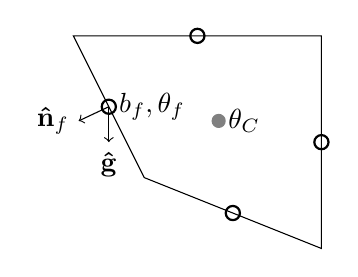
\begin{tikzpicture}[
  scale=0.45,
  cpnt/.style={fill=gray}
]

\draw (2,3) -- (0,7) -- (7,7) -- (7,1) -- (2,3);

\path [cpnt] (4.1,4.6) circle [radius=0.2] node [right] {$\theta_C$};

\draw [thick] (7,4) circle [radius=0.2];
\draw [thick] (4.5,2) circle [radius=0.2];
\draw [thick] (3.5,7) circle [radius=0.2];
\draw [thick] (1,5) circle [radius=0.2] node [right] {$b_f, \theta_f$};

\draw [->] (1,5) -- (0.15,4.6) node [left] {$\mathbf{\hat{n}}_f$};
\draw [->] (1,5) -- (1,4) node [below] {$\mathbf{\hat{g}}$};

\end{tikzpicture}
\end{document}

	\caption{A quadrilateral cell with the prognostic thermodynamic variable $b_f$ stored at face centres marked by open circles.
	$b_f$ is calculated from the potential temperature $\theta_f$ such that $b_f = \theta_f \unitg \cdot \unitn_f$ where $\unitn_f$ is the unit vector outward normal to face $f$, and $\unitg$ is the unit vector of gravitational acceleration.
	The potential temperature at the cell centre, $\theta_C$, is reconstructed from surrounding values of $b_f$ using equation~\eqref{eqn:cp:reconstruct}.}
	\label{fig:cp:staggering}
\end{figure}

The generalised Charney--Phillips model is a new variant of the fully compressible Euler model with a Lorenz staggering, as documented by \citet{weller-shahrokhi2014} and summarised in section~\ref{sec:slanted:exnerFoamH}.
The model variant uses a newly-formulated generalisation of the Charney--Phillips staggering for arbitrary meshes.
The primary difference between the Lorenz and Charney--Phillips formulations is their treatment of the prognostic thermodynamic variable: the generalised Charney--Phillips formulation stores the prognostic thermodynamic variable $b_f$ at all cell faces such that $b_f = \theta_f \unitg \cdot \unitn_f$ where $f$ is a face, $\theta_f$ is the potential temperature at the face, $\unitg$ is the unit vector of gravitational acceleration and $\unitn_f$ is the unit vector that is outward normal to the face.
This arrangement is illustrated in figure~\ref{fig:cp:staggering}.
To transport the thermal field, first, potential temperature is transported in advective form using first-order time-stepping,
\begin{align}
	\theta_f^{n+1} &= \theta_f^n - \Delta t \uf \cdot \left( \nabla_c \theta_f^{\ell} \right)_F \label{eqn:cp:advection}
\end{align}
where $\theta_f^{n+1}$ is the value of $\theta_f$ at the new time-step, $\theta_f^\ell$ is the lagged value from the previous time-stepping iteration, $\uf$ is the wind, $\left( \cdot \right)_F$ denotes an interpolation from cell centres to faces, and $\nabla_c$ denotes a cell centre gradient \citep{weller-shahrokhi2014}.
Next, $b_f$ is calculated such that $b_f = \theta_f \unitg \cdot \unitn_f$.  
On a Cartesian mesh with no diagonal faces, $b_f$ is zero for entirely vertical faces and $b_f = \theta_f$ for entirely horizontal faces.

Potential temperature at the cell centre is reconstructed from bordering faces,
\begin{align}
	\theta_C &= \unitg \cdot \left( \sum_{f \in c} \unitn_f \Sf \right)^{-1} \cdot \sum_{f \in c} \Sf b_f \label{eqn:cp:reconstruct}
\end{align}
where $\theta_C$ is the reconstructed potential temperature.  On a Cartesian mesh with no diagonal faces, $\theta_C$ is simply a linear interpolation from the face values immediately above and below the cell centre.

Finally, $\theta_f$ is recalculated from $b_f$ and $\theta_C$,
\begin{align}
	\theta_f &:= \Mag{ \unitg \cdot \unitn_f \theta_f} + \left( 1 - \Mag{\unitg \cdot \unitn_f } \right) \left( \theta_C \right)_F \text{.}
\end{align}
This ensures that values of $\theta_f$ on vertical faces is calculated from nearby $b_f$ values and is not retained across time-steps.

The generalised Charney--Phillips model variant makes two other modifications to the Lorenz model variant in order to simplify implementation: first, gravity waves are treated explicitly and, second, first-order Euler semi-implicit time-stepping is used with deferred correction of explicit terms (equation~\ref{eqn:cp:advection}).


\section{Transport over a mountainous lower boundary}
\label{sec:slanted:mountainAdvect}

The two-dimensional tests performed in chapter~\ref{ch:cubicFit} transported tracers positioned well above the terrain surface.  Here we formulate a new test, positioning the tracer at the ground in order to assess the accuracy of transport schemes immediately above a mountainous lower boundary.  Results using the cubicFit scheme are compared with the linearUpwind scheme on basic terrain-following, cut cell and slanted cell meshes.
The test presents a particular challenge to transport schemes as they must transport the tracer through arbitrarily small cut cells and distorted slanted cells.

The domain size and mountain profile is the same as those in the horizontal tracer advection test in section~\ref{sec:cubicFit:schaerAdvect}, with a mesh spacing of $\Delta x = \SI{1000}{\meter}$ and $\Delta z = \SI{500}{\meter}$.
Cell edges in the central region of the domain are shown in figure~\ref{fig:slanted:mountainAdvect:meshes} for each of the three mesh types.
Cells in the BTF mesh are highly distorted over steep slopes (figure~\ref{fig:slanted:mountainAdvect:meshes:btf}) while the cut cell mesh (figure~\ref{fig:slanted:mountainAdvect:meshes:cutCell}) and slanted cell mesh (figure~\ref{fig:slanted:mountainAdvect:meshes:slantedCell}) are orthogonal everywhere except for cells nearest the ground.

\begin{figure}
	\centering
	\begin{subfigure}{\textwidth}
		\phantomsubcaption\label{fig:slanted:mountainAdvect:meshes:btf}
		\phantomsubcaption\label{fig:slanted:mountainAdvect:meshes:cutCell}
		\phantomsubcaption\label{fig:slanted:mountainAdvect:meshes:slantedCell}
		\includegraphics{thesis/slanted/mountainAdvect/fig-meshes.pdf}
	\end{subfigure}
%
	\caption{Two dimensional $x$-$z$ meshes created with the (\subcaptionref{fig:slanted:mountainAdvect:meshes:btf}) basic terrain-following,
	(\subcaptionref{fig:slanted:mountainAdvect:meshes:cutCell}) cut cell, and
	(\subcaptionref{fig:slanted:mountainAdvect:meshes:slantedCell}) slanted cell methods, and used for the tracer transport tests in section~\ref{sec:slanted:mountainAdvect}.  Cell edges are marked by thin black lines.  The peak mountain height $h_0 = \SI{5}{\kilo\meter}$.
The velocity field is the same for all mesh types with streamlines marked on each panel by thick red lines.
The velocity field (equation~\ref{eqn:streamfunc-btf}) follows the lower boundary and becomes entirely horizontal above $H_1 = \SI{10}{\kilo\meter}$.
Only the lowest \SI{10}{\kilo\meter} for the central region of the domain is shown.  The entire domain is \SI{301}{\kilo\meter} wide and \SI{25}{\kilo\meter} high.}
	\label{fig:slanted:mountainAdvect:meshes}
\end{figure}

A velocity field is chosen that follows the terrain at the surface and becomes entirely horizontal above $H_1 = \SI{10}{\kilo\meter}$.
The value of $H_1$ is chosen to be much smaller than the domain height $H$ in equation~\eqref{eqn:btf} so that flow crosses the surfaces of the BTF mesh.
This is evident in figure~\ref{fig:slanted:mountainAdvect:meshes:btf} where the the velocity streamlines are tangential to the mesh only at the ground.
The flow is deliberately misaligned with the BTF, cut cell and slanted cell meshes away from the ground (figure~\ref{fig:slanted:mountainAdvect:meshes}) to ensure that flow always crosses mesh surfaces in order to challenge the transport schemes.

\begin{table}
	\centering
	\input{slanted/mountainAdvect/timesteps}
%
	\caption{Time-steps (\si{\second}) for the two-dimensional transport test over a mountainous lower boundary.  The time-steps were chosen so that the maximum Courant number was between \num{0.36} and \num{0.46}.}
	\label{tab:slanted:mountainAdvect:timesteps}
\end{table}

The tracer is defined again by equation~\eqref{eqn:cubicFit:schaerAdvect:tracer} but is now positioned at the ground with $(x_0, z_0) = (\SI{-50}{\kilo\meter}, \SI{0}{\kilo\meter})$ with half-widths $A_x = \SI{25}{\kilo\meter}$ and $A_z = \SI{10}{\kilo\meter}$.
Tests are integrated forward for \SI{10000}{\second}.  The time-step was chosen for each mesh so that the maximum Courant number was about \num{0.4} (table~\ref{tab:slanted:mountainAdvect:timesteps}).
An analytic solution at \SI{10000}{\second} is obtained by calculating the new horizontal position of the tracer using equation~\eqref{eqn:cubicFit:tfAdvect:trajectory}.
By solving this equation we find that \(x(t=\SI{10000}{\second}) = \TODO{\SI{123}{\meter}}\) when $h_0 = \SI{5}{\kilo\meter}$.

The tracer density boundary conditions are the same as those in section~\ref{sec:cubicFit:schaerAdvect}.
Since the cubicFit transport scheme uses values at boundaries with Dirichlet boundary conditions, the cubicFit scheme uses only inlet boundary values in this test case.

\begin{figure}
	\centering
	\includegraphics{thesis/slanted/mountainAdvect/fig-tracer.pdf}
	%
	\caption{Evolution of the tracer in the two-dimensional transport test over a mountainous lower boundary.  The tracer is transported to the right over the wave-shaped terrain.  Tracer contours are every \SI{0.1}{\kilo\gram\per\meter\cubed}.  The result obtained using the cubicFit scheme on the basic terrain-following mesh is shown at $t=\SI{0}{\second}$, $t=\SI{5000}{\second}$ and $t=\SI{10000}{\second}$ with solid black contours. The analytic solution at $t=\SI{10000}{\second}$ is shown with dotted contours.
	The shaded box indicates the region that is plotted in figure~\ref{fig:slanted:mountainAdvect:errors}.}
	\label{fig:slanted:mountainAdvect:tracer}
\end{figure}

Three series of tests were performed using similar configurations.  The first series uses a peak mountain height of $h_0 = \SI{5}{\kilo\meter}$ to examine errors on different mesh types using the two transport schemes.
The second series varies the peak mountain height to examine the sensitivity of the transport schemes to mesh distortions.
The third series verifies accuracy at Courant numbers close to the limit of stability, and examines the longest stable time-step for different mesh types.

\subsection{A comparison of numerical accuracy between mesh types and transport schemes}
For the first series of tests with $h_0 = \SI{5}{\kilo\meter}$, tracer contours at the initial time $t=\SI{0}{\second}$, half-way time $t=\SI{5000}{\second}$, and end time $t=\SI{10000}{\second}$ are shown in figure~\ref{fig:slanted:mountainAdvect:tracer} using the cubicFit scheme on the BTF mesh.  As apparent at $t=\SI{5000}{\second}$, the tracer is distorted by the terrain-following velocity field as it passes over the mountain, but its original shape is restored once it has cleared the mountain by $t=\SI{10000}{\second}$.
A small phase lag is apparent when the numerical solution marked with solid contour lines is compared with the analytic solution marked with dotted contour lines.

\begin{figure}
	\begin{subfigure}{\textwidth}
		\centering
		\phantomsubcaption\label{fig:slanted:mountainAdvect:errors:linearUpwind-btf}
		\phantomsubcaption\label{fig:slanted:mountainAdvect:errors:linearUpwind-cutCell}
		\phantomsubcaption\label{fig:slanted:mountainAdvect:errors:linearUpwind-slantedCell}
		\phantomsubcaption\label{fig:slanted:mountainAdvect:errors:cubicFit-btf}
		\phantomsubcaption\label{fig:slanted:mountainAdvect:errors:cubicFit-cutCell}
		\phantomsubcaption\label{fig:slanted:mountainAdvect:errors:cubicFit-slantedCell}
		%
		\includegraphics{thesis/slanted/mountainAdvect/fig-error.pdf}
	\end{subfigure}

	\caption{Tracer contours at $t=\SI{10000}{\second}$ for the two-dimensional tracer transport tests over a mountainous lower boundary.  A region in the lee of the mountain is plotted corresponding to the shaded area in figure~\ref{fig:slanted:mountainAdvect:tracer}.
	Results are presented on BTF, cut cell and slanted cell meshes (shown in figure~\ref{fig:slanted:mountainAdvect:meshes}) using the linearUpwind and cubicFit transport schemes.  The numerical solutions are marked by solid black lines.  The analytic solution is marked by dotted lines.  Contours are every \SI{0.1}{\kilo\gram\per\meter\cubed}.}
	\label{fig:slanted:mountainAdvect:errors}
\end{figure}

Numerical errors are more clearly revealed by subtracting the analytic solution from the numerical solution.
Error fields are compared between BTF, cut cell and slanted cell meshes using the linearUpwind scheme (figures~\ref{fig:slanted:mountainAdvect:errors:linearUpwind-btf},
\ref{fig:slanted:mountainAdvect:errors:linearUpwind-cutCell} and
\ref{fig:slanted:mountainAdvect:errors:linearUpwind-slantedCell} respectively) and the cubicFit scheme (figures~\ref{fig:slanted:mountainAdvect:errors:cubicFit-btf},
\ref{fig:slanted:mountainAdvect:errors:cubicFit-cutCell} and
\ref{fig:slanted:mountainAdvect:errors:cubicFit-slantedCell} respectively).
Results are least accurate using the linearUpwind scheme on the slanted cell mesh (figure~\ref{fig:slanted:mountainAdvect:errors:linearUpwind-slantedCell}) with the final tracer being slightly distorted.
The $\ell_\infty$ error magnitude is reduced by using the linearUpwind scheme on the cut cell mesh (figure~\ref{fig:slanted:mountainAdvect:errors:linearUpwind-cutCell}), but the shape of the error remains the same.
On the BTF mesh (figure~\ref{fig:slanted:mountainAdvect:errors:cubicFit-btf}), cut cell mesh (figure~\ref{fig:slanted:mountainAdvect:errors:cubicFit-cutCell}) and slanted cell mesh (figure~\ref{fig:slanted:mountainAdvect:errors:cubicFit-slantedCell}), the cubicFit scheme is more accurate than the linearUpwind scheme.

\subsection{Numerical stability and numerical accuracy with increasingly steep slopes}

\begin{figure}
	\centering
	\input{slanted/mountainAdvect/l2ByMountainHeight}
%
	\caption{Error measures for the two-dimensional tracer transport tests over a mountainous lower boundary.  Peak mountain heights $h_0$ are from \SIrange{0}{6}{\kilo\meter}.  Results are compared on BTF, cut cell and slanted cell meshes using the linearUpwind and the cubicFit schemes.  At $h_0 = \SI{0}{\kilo\meter}$ the terrain is entirely flat and the BTF, cut cell and slanted cell meshes are identical.  At $h_0 = \SI{6}{\kilo\meter}$ the linearUpwind scheme is unstable on the slanted cell mesh.}
	\label{fig:slanted:mountainAdvect:l2ByMountainHeight}
\end{figure}

To further examine the performance of the cubicFit scheme in the presence of steep terrain, a second series of tests were performed in which the peak mountain height was varied from \SIrange{0}{6}{\kilo\meter} keeping all other parameters constant.
Results were obtained on BTF, cut cell and slanted cell meshes using the linearUpwind scheme and cubicFit scheme.  Again, the time-step was chosen for each test so that the maximum Courant number was about \num{0.4} (table~\ref{tab:slanted:mountainAdvect:timesteps}).  The $\ell_2$ error was calculated by subtracting the analytic solution from the numerical solution (figure~\ref{fig:slanted:mountainAdvect:l2ByMountainHeight}).
Note that the analytic solution is a function of mountain height, with the tracer travelling farther over higher mountains due to non-divergent flow through a narrower channel.
In all cases, error increases with increasing mountain height because steeper slopes lead to greater mesh distortions.
Errors are identical for a given transport scheme when $h_0 = \SI{0}{\kilo\meter}$ and the ground is entirely flat because the BTF, cut cell and slanted cell meshes are identical.
Compared with the cubicFit scheme, the linearUpwind scheme is more sensitive to the mesh type and mountain height.  The linearUpwind scheme is unstable on the slanted cell mesh with a peak mountain height $h_0 = \SI{6}{\kilo\meter}$ despite using a Courant number of \inputval{mountainAdvect-h0-slantedCell-1000-6000m-linearUpwind/co}\unskip.
In contrast, the cubicFit scheme is less sensitive to the mesh type and errors grow more slowly with increasing mountain height.  The cubicFit scheme yields stable results in all tests.

\subsection{Numerical stability limits of the cubicFit transport scheme}

\begin{figure}
	\begin{subfigure}{\textwidth}
		\centering
		\input{slanted/mountainAdvect/maxdt}
		\phantomsubcaption\label{fig:slanted:mountainAdvect:maxdt:dt}
		\phantomsubcaption\label{fig:slanted:mountainAdvect:maxdt:co}
	\end{subfigure}
	%
	\caption{(\subcaptionref{fig:slanted:mountainAdvect:maxdt:dt}) Longest stable time-steps, $\Delta t_\mathrm{max}$, and 
	(\subcaptionref{fig:slanted:mountainAdvect:maxdt:co}) largest stable maximum Courant numbers, $\max(\mathrm{Co})$, for the two-dimensional tracer transport test over a mountainous lower boundary.  Results were obtained on basic terrain-following, cut cell and slanted cell meshes at mesh spacings between $\Delta x = \SI{5000}{\meter}$ and $\Delta x = \SI{250}{\meter}$.  The largest stable maximum Courant numbers were calculated from the corresponding longest stable time-steps using equation~\eqref{eqn:co}.}
	\label{fig:slanted:mountainAdvect:maxdt}
\end{figure}

A final series of tests were performed to determine the stability limit of the cubicFit scheme with the two-stage Heun time-stepping scheme (equation~\ref{eqn:heun}).
The tracer was transported on BTF, slanted cell and cut cell meshes with a variety of mesh spacings between $\Delta x = \SI{5000}{\meter}$ and $\Delta x = \SI{125}{\meter}$.  $\Delta z$ was chosen so that a constant aspect ratio is preserved such that $\Delta x / \Delta z = 2$.
For each test, the time-step was increased until the result became unstable.  The largest stable time-steps, $\Delta t_\mathrm{max}$, are presented in figure~\ref{fig:slanted:mountainAdvect:maxdt:dt}.
BTF meshes permit the longest time-steps of all three mesh types since cells are almost uniform in volume.  As expected, the longest stable time-step scales linearly with BTF mesh spacing.
There is no such linear scaling on cut cell meshes because these meshes can have arbitrarily small cells.  The time-step constraints on cut cell meshes are the most severe of the three mesh types.  Slanted cell meshes have a slightly stronger time-step constraint than BTF meshes but still exhibit similar linear scaling with mesh spacing.

Figure~\ref{fig:slanted:mountainAdvect:maxdt:co} presents the largest stable maximum Courant numbers, $\max(\mathrm{Co})$, which were calculated by substituting $\Delta t = \Delta t_\mathrm{max}$ into equation~\eqref{eqn:co}.
On basic terrain following meshes, the maximum Courant number tends towards about \num{1.3} with finer mesh spacings.
No such trend is found on cut cell or slanted cell meshes.
Cut cell meshes permit the largest maximum Courant numbers of around \num{3}, but the largest stable time-steps on cut cell meshes are still smaller than corresponding time-steps on basic terrain following and slanted cell meshes.

This thesis focuses on the spatial discretisation of the cubicFit scheme, but the stability limit depends also upon the choice of time-stepping.  We have not calculated a theoretical Courant number limit, although such an analysis should be possible using the techniques in \citep{baldauf2008}.

This new test case demonstrates that the cubicFit transport scheme is more accurate than the linearUpwind scheme on all meshes, and only the cubicFit scheme can achieve stable results on slanted cell meshes with very steep slopes.
The slanted cell method exhibits a time-step constraint that scales linearly with mesh spacing, and slanted cells avoid severe time-step constraints associated with arbitrarily small cut cells.
Next, we incorporate the cubicFit transport scheme into a model of the fully compressible Euler equations.

\section{Discretisation of the fully compressible Euler equations}
\label{sec:slanted:exnerFoamH}

The finite volume model of the fully compressible Euler equations is taken from \citet{weller-shahrokhi2014}, given by

\begin{subequations}
\begin{align}
	\text{Momentum} &\ &\  	\frac{\partial \rho \vect{u}}{\partial t} + \nabla \cdot \rho \vect{u}\otimes\vect{u} &= \rho \vect{g} - c_p \rho \theta \nabla \Pi - \mu \rho \vect{u} \label{eqn:exnerFoam:momentum} \\
	\text{Continuity} &\ &\	\frac{\partial \rho}{\partial t} + \nabla \cdot \rho \vect{u} &= 0 \label{eqn:exnerFoam:cont} \\
	\text{Thermodynamic equation} &\ &\ \frac{\partial \rho \theta}{\partial t} + \nabla \cdot \rho \vect{u} \theta &= 0 \label{eqn:exnerFoam:theta} \\
	\text{Ideal gas law} &\ &\ \Pi^{(1 - \kappa)/\kappa} &= \frac{R \rho \theta}{p_0} \label{eqn:exnerFoam:state}
\end{align}
\end{subequations}
where \(\rho\) is the density, \(\vect{u}\) is the velocity field, \(\vect{g}\) is the gravitational acceleration, \(c_p\) is the heat capacity at constant pressure, \(\theta = T \left(p_0/p\right)^\kappa\) is the potential temperature, \(T\) is the temperature, \(p\) is the pressure, \(p_0 = \SI{1000}{\hecto\pascal}\) is a reference pressure, \(\Pi = \left(p / p_0 \right)^\kappa\) is the Exner function of pressure, and \(\kappa = R/c_p\) is the gas constant to heat capacity ratio.  \(\mu\) is a damping function that can be used to absorb momentum near the upper boundary.

The model uses the C-grid staggering in the horizontal and the Lorenz staggering in the vertical such that $\theta$, $\rho$ and $\Pi$ are stored at cell centroids and the covariant component of velocity at cell faces.  The model is configured without Coriolis forces.

Acoustic and gravity waves are treated implicitly and transport terms are treated explicitly.
The trapezoidal implicit treatment of fast waves and the Hodge operator suitable for non-orthogonal meshes are described in the appendix to \citet{shaw-weller2016}.
To avoid time-splitting errors between transport and fast waves, transport is time-stepped using a three-stage, second-order Runge-Kutta scheme.
The transport terms of the momentum equation \eqref{eqn:exnerFoam:momentum} and thermodynamic equation \eqref{eqn:exnerFoam:theta} are discretised in flux form using the cubicFit transport scheme.

This model is suitable for arbitrary meshes and includes a curl-free pressure gradient formulation.
In the next section, we use this model to compare the accuracy of pressure gradient calculations using terrain-following, cut cell and slanted cell meshes.

\section{Stratified atmosphere initially at rest}
\label{sec:slanted:resting}

Diurnal valley and slope flows are associated with weak synoptic-scale winds, and cold air that sinks along sloping terrain can stagnate for days after becoming trapped in topographic basins \citep{chow2013}.
The test case by \citet{klemp2011} is an idealised representation of such phenomena, in which a wave-shaped mountain is submerged in a stably stratified atmosphere at rest in hydrostatic balance.
The analytic solution is time-invariant, but numerical errors in calculating pressure gradients can give rise to spurious flows which become stronger over steeper terrain \citep{klemp2011}.
Results are compared using terrain-following, cut cell and slanted cell meshes.

Following \cite{klemp2011}, the domain is \SI{200}{\kilo\meter} wide and \SI{20}{\kilo\meter} high, and the mesh spacing is \(\Delta x = \Delta z^\star = \SI{500}{\meter}\).  All boundary conditions are no normal flow.
The wave-shaped mountain profile has a surface height, $h$, given by
\begin{align}
	h(x) = h_0 \exp \left( - \left( \frac{x}{a} \right)^2 \right) \cos^2 \left( \alpha x \right) \label{eqn:resting:mountain}
\end{align}
where $a = \SI{5}{\kilo\meter}$ is the mountain half-width $\lambda = \SI{4}{\kilo\meter}$ is the wavelength and $h_0$ is the peak mountain height.  For the optimised SLEVE mesh, the coarse-scale component $h_1$ is specified as
\begin{align}
	h_1(x) = \frac{1}{2} h_0 \exp \left( - \left( \frac{x}{a} \right)^2 \right) \text{ .}
\end{align}
To accommodate a range of mountain heights we choose a coarse scale height $s_1 = \SI{20}{\kilo\meter}$ and a fine scale height $s_2 = \SI{8}{\kilo\meter}$.  Following \citet{leuenberger2010} the optimal exponent value of $n = \num{1.35}$ is used.  These parameter values result in a SLEVE mesh that is more distorted than the SLEVE mesh used by \citet{klemp2011}, but the choice is necessary to avoid mesh tangling with mountains higher than \SI{1}{\kilo\meter}.

The initial potential temperature field has a nonlinear vertical profile in the lower atmosphere, with $\theta(z = 0) = \SI{288}{\kelvin}$ and a constant static stability with Brunt-V\"ais\"al\"a frequency $N = \SI{0.01}{\per\second}$ everywhere, except for a more stable layer of $N = \SI{0.02}{\per\second}$ between $\SI{2}{\kilo\meter} \leq z \leq \SI{3}{\kilo\meter}$.
The Exner function of pressure is calculated so that it is in discrete hydrostatic balance in the vertical direction \citep{weller-shahrokhi2014}.

Momentum and potential temperature are transported using the cubicFit transport scheme.
The damping function \(\mu\) is set to \SI{0}{\per\second}.  Unlike \citet{klemp2011}, there is no eddy diffusion in the equation set.

\begin{figure}
	\centering
	\begin{subfigure}{\textwidth}
		\centering
		\input{slanted/resting/w}
		\phantomsubcaption\label{fig:slanted:resting:w:timeseries}
		\phantomsubcaption\label{fig:slanted:resting:w:max}
	\end{subfigure}
	\caption{Spurious vertical velocities in the resting atmosphere test using BTF, SLEVE, cut cell and slanted cell meshes.
	(\subcaptionref{fig:slanted:resting:w:timeseries}) Time series of spurious vertical velocities for a peak mountain height $h_0 = \SI{1}{\kilo\meter}$, with the maximum absolute value calculated at each time-step. 
	(\subcaptionref{fig:slanted:resting:w:max}) Sensitivity to peak mountain height $h_0$, with the maximum absolute value calculated across all time-steps.
	}
	\label{fig:slanted:resting:w}
\end{figure}

The test is integrated forward by \num{6} hours using a time-step of $\Delta t = \SI{25}{\second}$ on the BTF, SLEVE, cut cell and slanted cell meshes with a peak mountain height $h_0 = \SI{1}{\kilo\meter}$.
For each mesh, the maximum absolute vertical velocity is calculated at each time-step as a measure of the spurious flow generated by numerical errors.  In agreement with \citep{klemp2011}, magnitudes of vertical velocity peak shortly after integration begins and magnitudes are larger on more distorted meshes (figure~\ref{fig:slanted:resting:w:timeseries}).
However, magnitudes are much smaller comparing results on the terrain-following meshes with those from \citet{klemp2011}: results in figure~\ref{fig:slanted:resting:w:timeseries}, which use a curl-free pressure gradient formulation, have maximum absolute vertical velocities of \inputval{resting-btf-1000m-cubicFit/maxw}\unskip, compared with a maximum of $\sim \SI{7}{\meter\per\second}$ found by \citet{klemp2011} using their improved horizontal pressure gradient formulation.
The results on terrain-following meshes in figure~\ref{fig:slanted:resting:w:timeseries} have similar maximum errors as \citet{weller-shahrokhi2014} but, due to the more stable split into implicitly and explicitly treated terms (described in the appendix to \citet{shaw-weller2016}), the errors decay over time due to the dissipative nature of the transport scheme.
Unlike the result from \citet{klemp2011}, spurious flows are similar on both terrain-following meshes even though the SLEVE mesh is less distorted than the BTF mesh.

Compared to results on the terrain-following meshes, spurious flows are two orders of magnitude smaller on the cut cell mesh and the slanted cell mesh with a maximum absolute vertical velocity of $\sim \SI{1e-3}{\meter\per\second}$.
\citet{good2014} found the maximum vertical velocity in their cut cell model was \SI{1e-12}{\meter\per\second}, which is better than any result obtained here.  It is worth noting that our model stores values at the geometric centre of cut cells, whereas the model used by \citet{good2014} has cell centres at the centre of the uncut cell, resulting in the centre of some cut cells being below the ground (S.-J. Lock 2014, personal communication).
This means that the mesh is effectively regular when calculating horizontal and vertical gradients, and this would account for the very small velocities found by \citet{good2014}.

To evaluate the slanted cell method with steeper slopes, we perform a second series of tests with peak mountain heights ranging from $h_0 = \SI{0}{\kilo\meter}$ to $h_0 = \SI{6}{\kilo\meter}$.
The BTF, SLEVE, cut cell and slanted cell meshes with the largest peak mountain height of $h_0 = \SI{6}{\kilo\meter}$ are shown in figure~\ref{fig:slanted:resting:meshes}.
To obtain a single measure of spurious flow for a given mesh, the maximum absolute vertical velocity is calculated across all time-steps.
The most accurate results are obtained without mountains when $h_0 = \SI{0}{\kilo\meter}$ when all meshes become identical, with $\max(\Mag{w}) \sim \SI{1e-11}{\meter\per\second}$.
Using terrain-following meshes, the model becomes unstable beyond $h_0 = \SI{2}{\kilo\meter}$.
Using cut cell meshes, maximum vertical velocities are almost constant at $\sim \SI{0.5}{\meter\per\second}$ beyond $h_0 = \SI{1}{\kilo\meter}$ because cut cell mesh distortions are largely independent of mountain height.
Using slanted cell meshes, maximum vertical velocities are one to two orders of magnitude smaller than those found on terrain-following meshes at a given mountain height.  Unlike results on terrain-following meshes, slanted cell meshes yield stable results for all mountain heights, although maximum vertical velocities increase with peak mountain height as slanted cells become increasingly distorted.  Up to a peak mountain height of $h_0 = \SI{4}{\kilo\meter}$, slanted cell meshes produce results that are more accurate than those obtained for any other mesh.

In summary, spurious velocities in the resting atmosphere test were similar on both types of terrain-following mesh, with errors being much smaller compared to those from \citet{klemp2011}.
The maximum absolute vertical velocity was decreased by one to two orders of magnitude using cut cell and slanted cell meshes so we conclude that, in this test, mesh distortion, or lack of alignment of the mesh with surfaces of constant gravitational potential, is the primary cause of numerical error.
The resting atmosphere test presented a challenge to the pressure gradient formulation but the resultant spurious flows presented no particular challenge to the cubicFit transport scheme.  We will turn our attention to transport-dominated flow in the next chapter.


\chapter{Generalising the Charney–Phillips staggering for arbitrary meshes}

\appendixpage
\appendix
\input{cubicFit/vonNeumann}
\section{Spherical corrections}
The Cartesian position vector $\bm{x} = (x,y,z)$ is related to the spherical coordinates $(\lon, \lat)$ by
\begin{align}
	(x,y,z) = (\Rearth \cos \lat \cos \lon, \Rearth \cos \lat \sin \lon, \Rearth \sin \lat) \label{eqn:spherical:cartesian}
\end{align}

\subsection{Velocity field specification}
The divergent velocity field in section~\ref{sec:deformationSphere:divergent} is specified as
\begin{align}
	\bm{u}(\lon, \lat, \Rearth) = \left[ 
	u(\lon, \lat, \Rearth),
	v(\lon, \lat, \Rearth),
	w(\lon, \lat, \Rearth)
	\right]^\transpose
\end{align}
given in local Cartesian coordinates on a plane tangent to the sphere at position $\bm{p} = \left[ \lon, \lat, \Rearth \right]^\transpose$.  Position $\bm{p}$ can be expressed in global Cartesian coordinates using equation~\eqref{eqn:spherical:cartesian}.
The velocity vector can be expressed in global Cartesian coordinates using the unit vectors of the tangent plane,
\begin{align}
	\unitlon = \left[ \hat{\lon}_x, \hat{\lon}_y, \hat{\lon}_z \right]^\transpose \\
	\unitlat = \left[ \hat{\lat}_x, \hat{\lat}_y, \hat{\lat}_z \right]^\transpose \\
	\unitradius = \left[ \hat{r}_x, \hat{r}_y, \hat{r}_z \right]^\transpose
\end{align}
which are themselves expressed in global Cartesian coordinates.
The radial unit vector $\unitradius$ is calculated first and is simply $\unitradius = \bm{p} / \Mag{\bm{p}}$.
The latitudinal unit vector $\unitlat$ is calculated next.  If $\unitradius$ points towards one of the Earth's poles then $\Mag{\unitk \times \unitradius} = 0$ where $\unitk = \left[0, 0, 1\right]^\transpose$ is the unit vector pointing to the North pole.
In this case, $\bm{\hat{\lat}} = \sign(\unitk \cdot \unitradius) \left[1, 0, 0\right]^\transpose$.  Otherwise, when $\unitradius$ does not point to a pole then
\begin{align}
	\bm{\hat{\lat}} = \frac{\unitradius \times \left( \unitk \times \unitradius \right)}{\Mag{\unitradius \times \left( \unitk \times \unitradius \right)}}
\end{align}
The longitudinal unit vector $\unitlon = \unitlat \times \unitradius$.
Finally, the velocity vector expressed in global Cartesian coordinates is
\begin{align}
	\bm{u}(x, y, z) = 
	\begin{bmatrix}
		\unitlon &
		\unitlat &
		\unitradius
	\end{bmatrix}^{-1}
	\bm{u}(\lon, \lat, \Rearth)
\end{align}



\backmatter
\bibliographystyle{ametsoc2014}
\bibliography{src/thesis/thesis}

\end{document}
